\chapter{Preliminaries}

A cellular automaton (CA) is a regular lattice of computational units called cells. Each cell $v$ is characterised by a state variable $S_i(t) \in \Sigma$, where $i$ indicates the position of the cell in the lattice, $t$ indicates the time, and $\Sigma$ denotes the (possibly infinite) set of all state variables. Each cell also has a finite local neighbourhood set $\mathcal{N}(v)$ with cardinality $N$. Typically, the neighbourhood of a cell contains the cell itself (i.e. $v \in \mathcal{N}(v)$). At each time step, the state of every cell is simultaneously updated according to a fixed transition rule; $\phi:\Sigma^N \to \Sigma$ which takes the neighbour states as input. This rule is typically shared across all cells in the CA.\\

The choice of neighbourhood function is largely directed by the choice of lattice structure. The primary considerations when choosing a neighbour function are the distance metric used to measure proximity of cells and the value of this metric used to define the neighbourhood boundary. There are two very common neighbourhoods used on Euclidean lattices. The \textit{von Neumann neighbourhood} contains all cells within a Manhattan distance of 1. For a 2D square lattice, this contains the cell itself and the 4 cells in the cardinal directions. For a 3D cubic lattice, it contains the central cell and a 6-cell octahedron around it. The \textit{Moore neighbourhood} contains all cells at a Chebyshev distance of 1. For a 2D square lattice, this is the central cell with the 8 neighbouring cells in a square around it. In the 3D case, it is a cube. These are shown in figure \ref{fig:neighbourhoods}

\begin{figure}[!h]
\centering
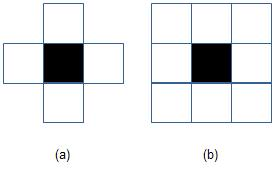
\includegraphics[width=0.5\textwidth]{images/neighbourhoods.png}
\caption{(a) von Neumann Neighbourhood and (b) Moore neighbourhood on a 2D square lattice \cite{debasis2011survey}}
\label{fig:neighbourhoods}
\end{figure}

\section{Conway's Game of Life}
The most popular example of a CA is the Game of Life (henceforth "Life") formulated by John Conway in 1970 \cite{gardner1970fantastic}. It consists of a 2D grid of cells, each with a boolean state variable signifying that the cell is either "alive" or "dead". The transition rule is a function of the cell's own state $S_i(t)$ and the number of living individuals in the cell's Moore neighbourhood (excluding itself), denoted $n$. This is as follows:

\begin{equation}
  \phi(S_i(t), n) = 
\begin{cases}
  0 & S_i(t) = 1 \text{ and } n < 2 \text{  (Death by "loneliness")}\\
  0 & S_i(t) = 1 \text{ and } n > 3 \text{  (Death by "overcrowding")}\\
  1 & S_i(t) = 1 \text{ and } n \in \{2,3\} \text{  (Survival)}\\
  1 & S_i(t) = 0 \text{ and } n = 3 \text{  (Resurrection)}\\
  0 & \text{otherwise}
\end{cases}
\end{equation}

Despite its simplicity, Life is Turing complete. There has been a lot of experimentation with Life to discover and classify patterns that can exist within it. Some examples include periodic oscillators like the \textit{beacon} which has period 2 or still lifes like the \textit{block} which are fixed-point solutions \ref{fig:life-patterns}. These can alternatively be thought of as having period 1. There are also periodic patterns that move across the lattice such as the \textit{glider} pattern.

\begin{figure}[!h]
\centering
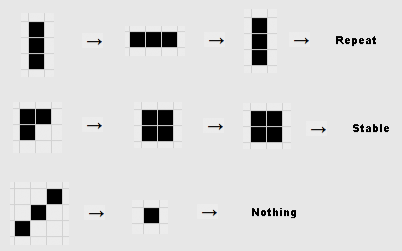
\includegraphics[width=0.8\textwidth]{images/life-patterns.png}
\caption{Patterns within the Game of Life. From top to bottom: blinker, block, unnamed \cite{lipa}}
\label{fig:life-patterns}
\end{figure}


\begin{figure}[!h]
\centering
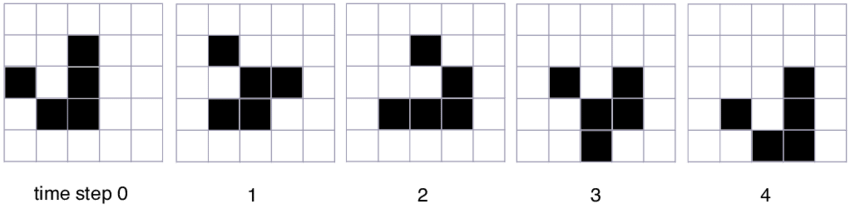
\includegraphics[width=0.8\textwidth]{images/life-glider.png}
\caption{The glider pattern within the Game of Life \cite{dorin2012framework}}
\label{fig:life-glider}
\end{figure}

\section{Wolfram's Classification}

The choices of lattice geometry, neighbourhood function, state variable, and transition rule define the behaviour of a CA. Fixing the former three factors, Wolfram \cite{wolfram1986theory} has classified CAs based on transition rules as follows:
\begin{enumerate}
  \item Class 1 (Null) : Rules that lead to a trivial, uniform state
  \item Class 2 (fixed-point + periodic) : Rules that lead to stable or periodic patterns
  \item Class 3 (Chaotic) : Rules that lead to chaotic patterns
  \item Class 4 (Complex) : Rules that lead to complex, long-lived impermanent patterns
\end{enumerate}

\textbf{Elementary cellular automata} are defined on the simplest nontrivial lattice, a finite one-dimensional chain. The neighbourhood of each cell contains the cell itself and the two cells adjacent to it on either side. The state variable is a boolean which means there are $2^3 = 8$ possible neighbourhood state configurations. A transition rule maps each of these neighbourhood states to a resultant state and can therefore be represented as an 8-digit binary rule table $(t_7t_6t_5t_4t_3t_2t_1t_0)$ where configuration $(000)$ maps to $t_0$, $(001)$ maps to $t_1$, ..., and $(111)$ maps to $(t_7)$. Consequently there are $2^8=256$ possible transition functions for elementary CA. Figure \ref{fig:rule-space} illustrates the distribution of classes in this rule space as we vary $p$, the proportion of 1s in the rule table. \\

The Wolfram code, a number between 0 and 255 obtained by converting the binary rule table to decimal, is the standard naming convention for these rules. Rule 110 is particularly notable as it can exhibit class 4 behaviour \cite{wolfram2002} and has been proven to be Turing Complete \cite{cook2004universality}. Figure \ref{fig:rule-110} shows an example progression of a Rule 110 system. Each row of pixels represents the state of the automaton at one snapshot in time with the topmost row representing the randomized initial state. It shows the emergence, interaction, and subsequent dissipation of multiple long-lived impermanent patterns.

\begin{figure}[!h]
\centering
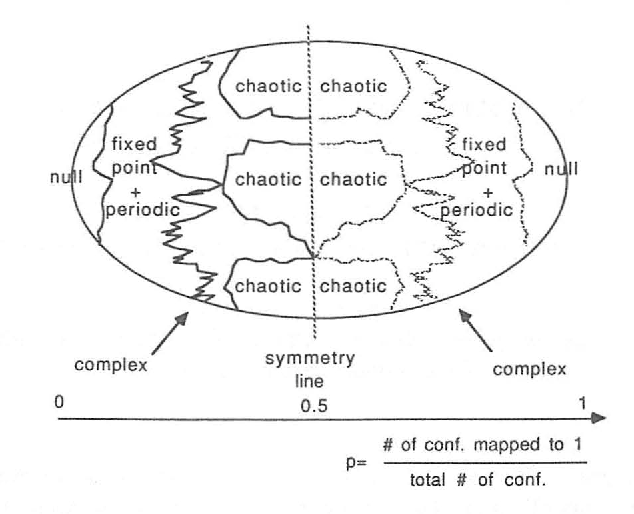
\includegraphics[width=0.9\textwidth]{images/rule-space.png}
\caption{Schematic illustration of elementary CA rule space from Li and Packard \cite{li1990structure}}
\label{fig:rule-space}
\end{figure}

\begin{figure}[!h]
\centering
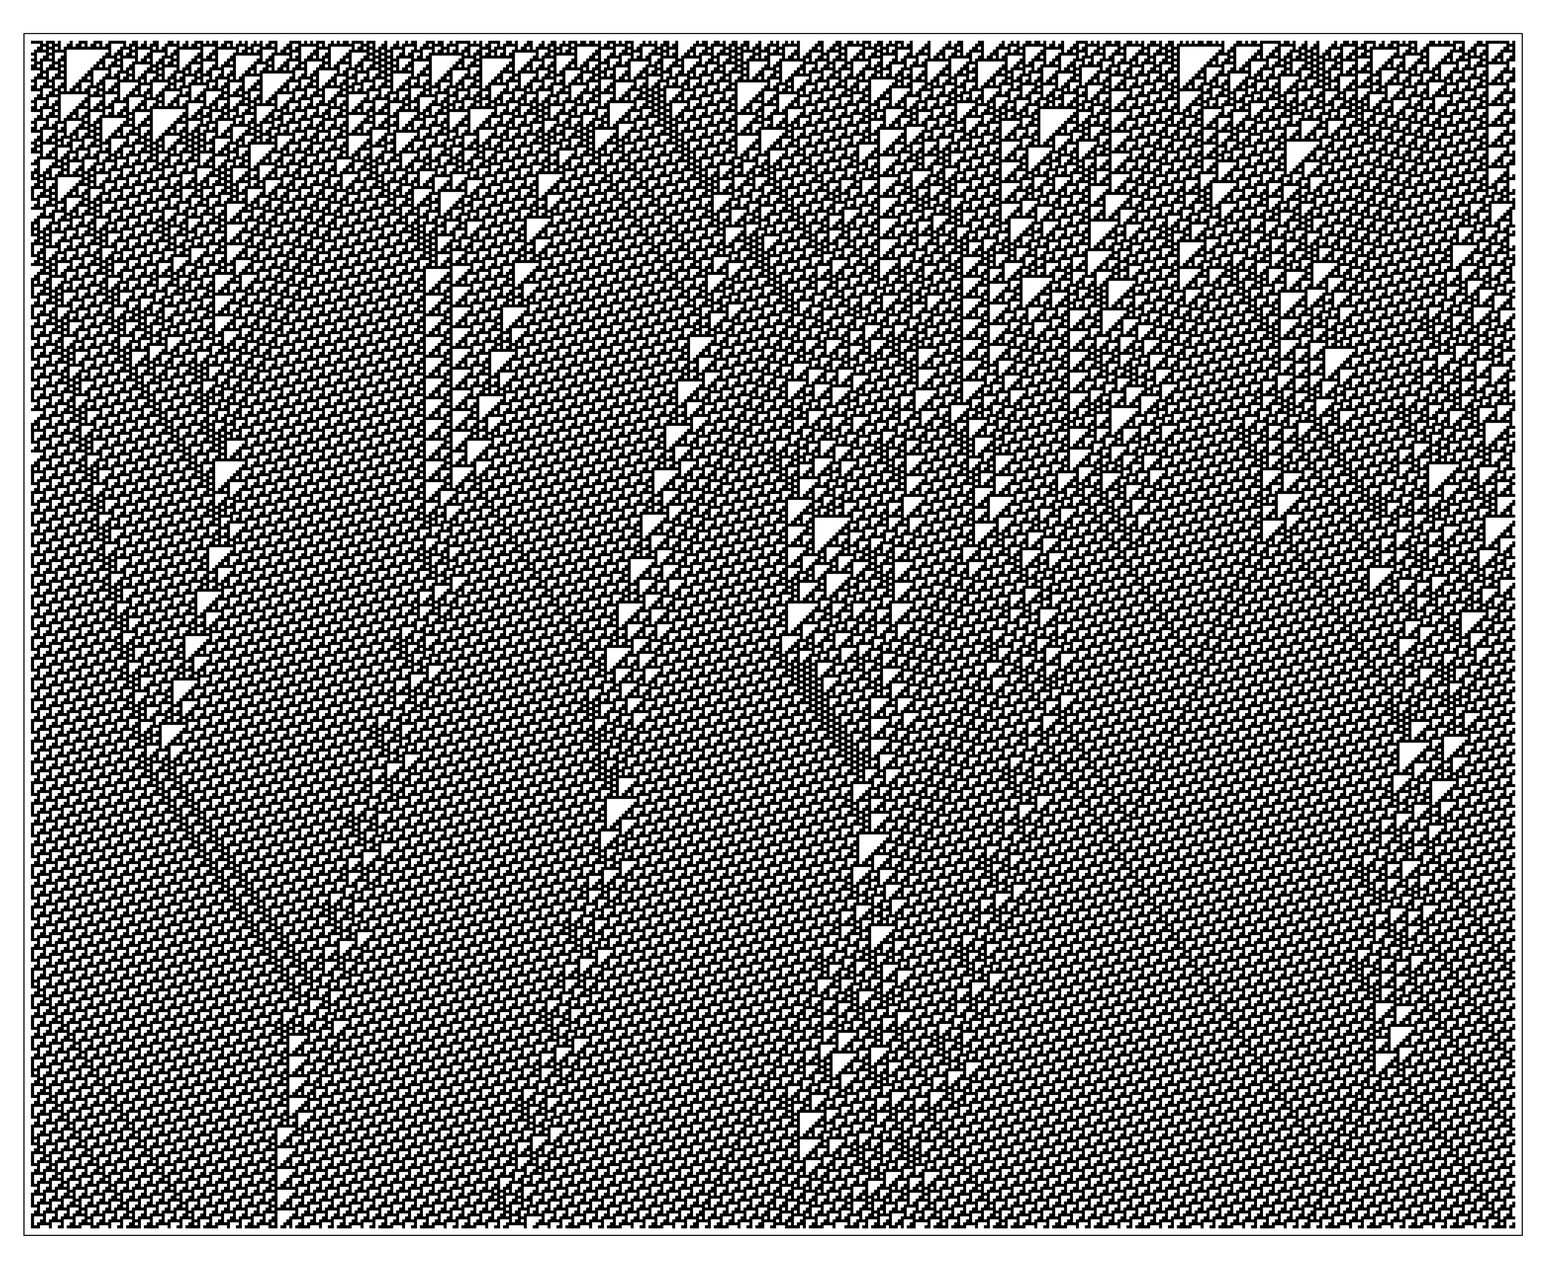
\includegraphics[width=0.9\textwidth]{images/rule-110.png}
\caption{Rule 110 progression with random initialisation \cite{wolfram2002}}
\label{fig:rule-110}
\end{figure}

\section{Morphogenesis}
Morphogenesis is the process by which a system develops into a particular shape or pattern. 
Biologically, this is seen in most multicellular organisms which can robustly develop specialised organs and intricate skin patterns without any centralised decision-making.
Through simple rules encoded in the genome and homeostatic feedback loops enforced through chemical signalling, a tissue knows exactly how to grow and when to stop.\\

Emulating this behaviour \textit{in silico} can provide great insight into the way self-organising and self-repairing biological systems function.
Cellular automata are a promising model of computation for artificial life simulation because, much like biological agents, their behaviour follows logically from combining information in their surroundings and internal programming.
In the context of morphogenesis, we are interested in rules that form stable class 2 patterns from random initial conditions.
We are also interested in rules that are resistant to noise.
This is analogous to the behaviour of biological cells which grow into stable configurations and are robust to perturbation and damage during growth.

% \section{Neural Networks}
% This section explores different categories of artificial neural networks that have been used to learn transition rules for cellular automata.

% \subsection{Convolutional Neural Networks}
% A convolutional neural network is an ANN that is particularly well-suited to inputs in grid-based topologies such as images and videos.
% Instead of containing fully connected layers, the neurons in the hidden layers of a CNN only take input from a particular receptive field.
% This design decision is broadly inspired by the way biological vision systems work.
% Cortical neurons respond only to light hitting a subset of the visual field and there is major overlap between the receptive fields of these neurons.\\

% A CNN architecture typically features two broad stages, embedding and classification. 
% The embedding stage features convolution, activation, and pooling operations.
% The classification stage usually contains fully connected layers.\\

% Convolution layers apply a dot product between a shared kernel matrix and a sub-grid of the input. 
% The kernel filter slides all such sub-grids and applies the convolution operation to produce an activation map.
% An activation function is then applied to each pixel in the activation map to introduce nonlinearity.
% Examples include the Sigmoid, Tanh, and ReLU functions.
% Pooling layers extract key information from sub-grids. Typical pooling operations include max-pooling, average-pooling, and L2 norm pooling. Each one extracts a single value from a kernel filter.\\

% \subsection{Graph Neural Networks}


% \subsection{Recurrent Neural Networks}

% \section{Mesh Construction}